% A simple graph with straight and bend arrows and loops
% Stefan Kottwitz
\documentclass{article}

\usepackage{tikz}
\usetikzlibrary{arrows}


\begin{document}



% graphe0.png : exemple
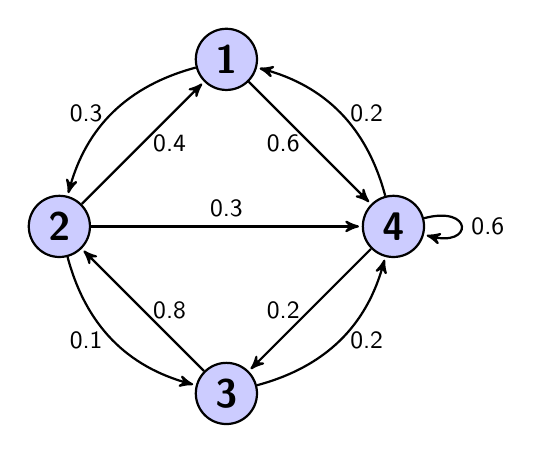
\begin{tikzpicture}[->,>=stealth',shorten >=1pt,auto,node distance=3cm,
  thick,main node/.style={circle,fill=blue!20,draw,font=\sffamily\Large\bfseries}]

  \node[main node] (1) {1};
  \node[main node] (2) [below left of=1] {2};
  \node[main node] (3) [below right of=2] {3};
  \node[main node] (4) [below right of=1] {4};

  \path[every node/.style={font=\sffamily\small}]
    (1) edge node [left] {0.6} (4)
        edge [bend right] node[left] {0.3} (2)
    (2) edge node [right] {0.4} (1)
        edge node {0.3} (4)
        edge [bend right] node[left] {0.1} (3)
    (3) edge node [right] {0.8} (2)
        edge [bend right] node[right] {0.2} (4)
    (4) edge node [left] {0.2} (3)
        edge [loop right] node {0.6} (4)
        edge [bend right] node[right] {0.2} (1);
\end{tikzpicture}



\vspace{2cm}
% graphe1.png : orienté

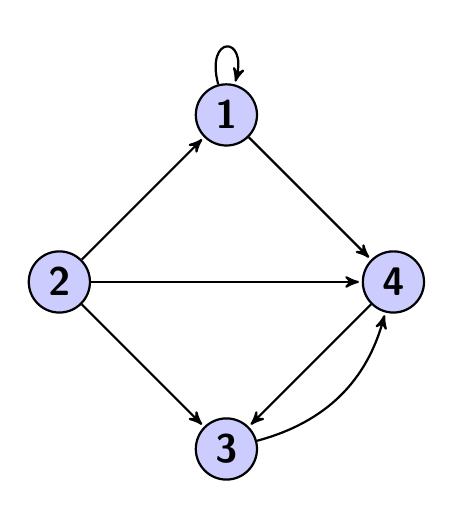
\begin{tikzpicture}[->,>=stealth',shorten >=1pt,auto,node distance=3cm,
  thick,main node/.style={circle,fill=blue!20,draw,font=\sffamily\Large\bfseries}]

  \node[main node] (1) {1};
  \node[main node] (2) [below left of=1] {2};
  \node[main node] (3) [below right of=2] {3};
  \node[main node] (4) [below right of=1] {4};

  \path[every node/.style={font=\sffamily\small}]
    (1) edge node [left] {} (4)
        edge [loop above] node {} (1)
    (2) edge node [right] {} (1)
        edge node {} (4)
        edge [right] node[left] {} (3)
    (3) edge [bend right] node[right] {} (4)
    (4) edge node [left] {} (3);
\end{tikzpicture}





\vspace{2cm}
% graphe2.png : non orienté

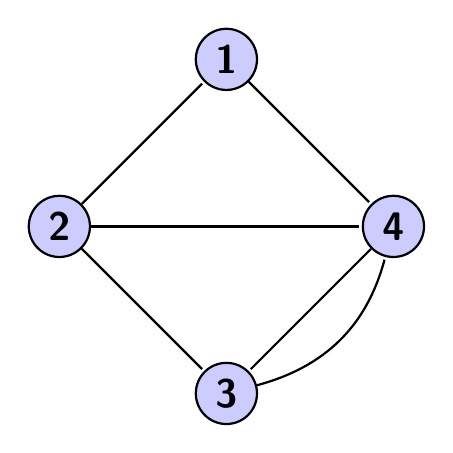
\begin{tikzpicture}[>=stealth',shorten >=1pt,auto,node distance=3cm,
  thick,main node/.style={circle,fill=blue!20,draw,font=\sffamily\Large\bfseries}]

  \node[main node] (1) {1};
  \node[main node] (2) [below left of=1] {2};
  \node[main node] (3) [below right of=2] {3};
  \node[main node] (4) [below right of=1] {4};

  \path[every node/.style={font=\sffamily\small}]
    (1) edge node [left] {} (4)
    (2) edge node [right] {} (1)
        edge node {} (4)
        edge [right] node[left] {} (3)
    (3) edge [bend right] node[right] {} (4)
    (4) edge node [left] {} (3);
\end{tikzpicture}





\vspace{2cm}
% graphe3.png : pondéré (exemple carte routière)

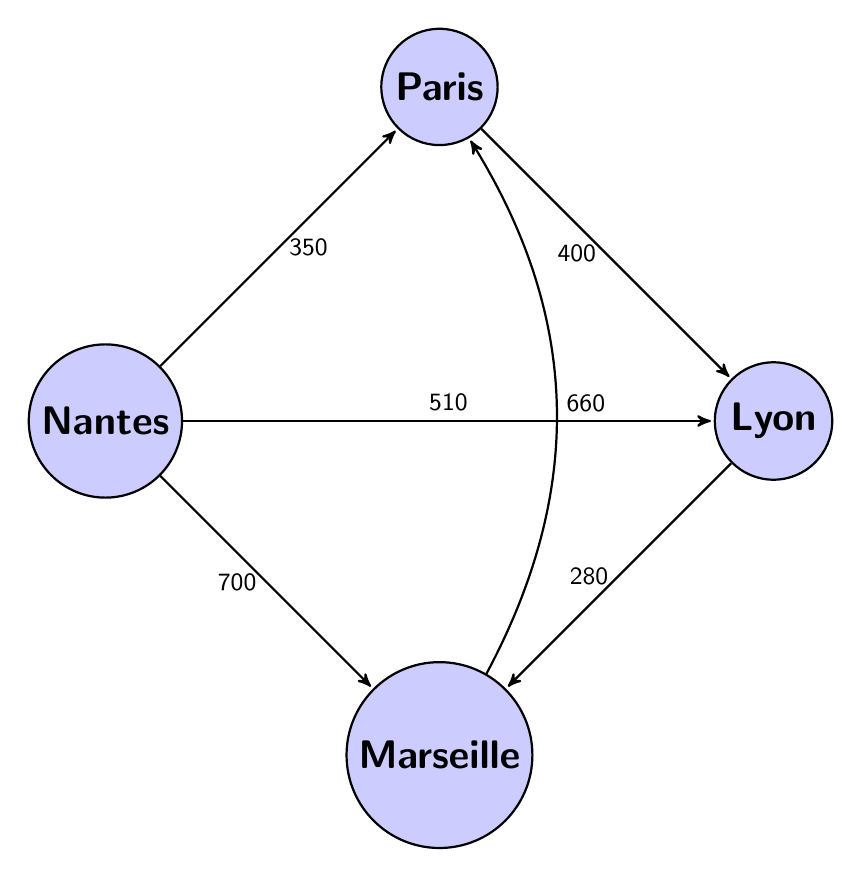
\begin{tikzpicture}[->,>=stealth',shorten >=1pt,auto,node distance=6cm,
  thick,main node/.style={circle,fill=blue!20,draw,font=\sffamily\Large\bfseries}]

  \node[main node] (1) {Paris};
  \node[main node] (2) [below left of=1] {Nantes};
  \node[main node] (3) [below right of=2] {Marseille};
  \node[main node] (4) [below right of=1] {Lyon};

  \path[every node/.style={font=\sffamily\small}]
    (1) edge node [left] {400} (4)
    (2) edge node [right] {350} (1)
        edge node {510} (4)
        edge [right] node[left] {700} (3)
    (3) edge [bend right] node[right] {660} (1)
    (4) edge node [left] {280} (3);
\end{tikzpicture}




\vspace{2cm}
% graphe4.png : cyclique

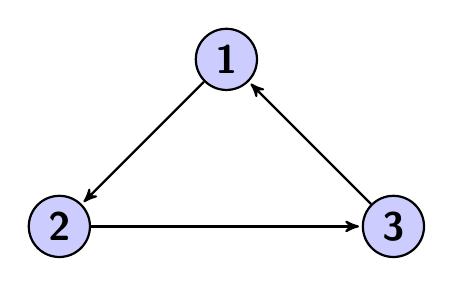
\begin{tikzpicture}[->,>=stealth',shorten >=1pt,auto,node distance=3cm,
  thick,main node/.style={circle,fill=blue!20,draw,font=\sffamily\Large\bfseries}]

  \node[main node] (1) {1};
  \node[main node] (2) [below left of=1] {2};
  \node[main node] (3) [below right of=1] {3};

  \path[every node/.style={font=\sffamily\small}]
    (1) edge node [right] {} (2)
    (2) edge node {} (3)
    (3) edge node [left] {} (1);
\end{tikzpicture}


\vspace{2cm}
% graphe5.png : acyclique

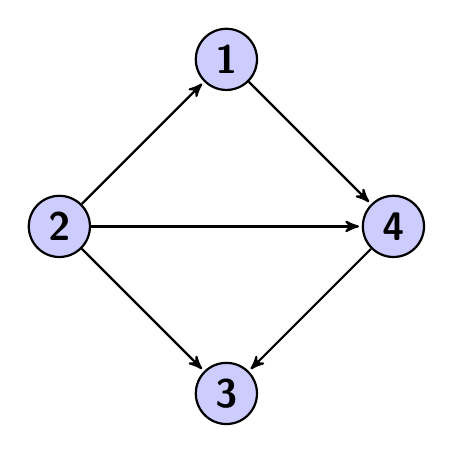
\begin{tikzpicture}[->,>=stealth',shorten >=1pt,auto,node distance=3cm,
  thick,main node/.style={circle,fill=blue!20,draw,font=\sffamily\Large\bfseries}]

  \node[main node] (1) {1};
  \node[main node] (2) [below left of=1] {2};
  \node[main node] (3) [below right of=2] {3};
  \node[main node] (4) [below right of=1] {4};

  \path[every node/.style={font=\sffamily\small}]
    (1) edge node [left] {} (4)
    (2) edge node [right] {} (1)
        edge node {} (4)
        edge [right] node[left] {} (3)
    (4) edge node [left] {} (3);
\end{tikzpicture}

\vspace{2cm}
% graphe6.png : dense

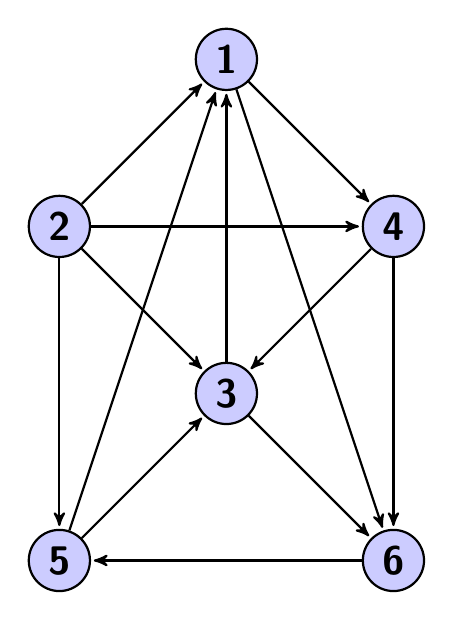
\begin{tikzpicture}[->,>=stealth',shorten >=1pt,auto,node distance=3cm,
  thick,main node/.style={circle,fill=blue!20,draw,font=\sffamily\Large\bfseries}]

  \node[main node] (1) {1};
  \node[main node] (2) [below left of=1] {2};
  \node[main node] (3) [below right of=2] {3};
  \node[main node] (4) [below right of=1] {4};
  \node[main node] (5) [below left of=3] {5};  
  \node[main node] (6) [below right of=3] {6};

  \path[every node/.style={font=\sffamily\small}]
    (1) edge node [left] {} (4)
        edge node [left] {} (6)
    (2) edge node [right] {} (1)
        edge node {} (4)
        edge [right] node[left] {} (3)
        edge node [right] {} (5)
    (3) edge node [right] {} (1)
        edge node [right] {} (6)
    (4) edge node [left] {} (3)
        edge node [right] {} (6)
    (5) edge node [right] {} (1)
        edge node [right] {} (3)
    (6) edge node [right] {} (5);
\end{tikzpicture}

\vspace{2cm}
% graphe7.png : creux

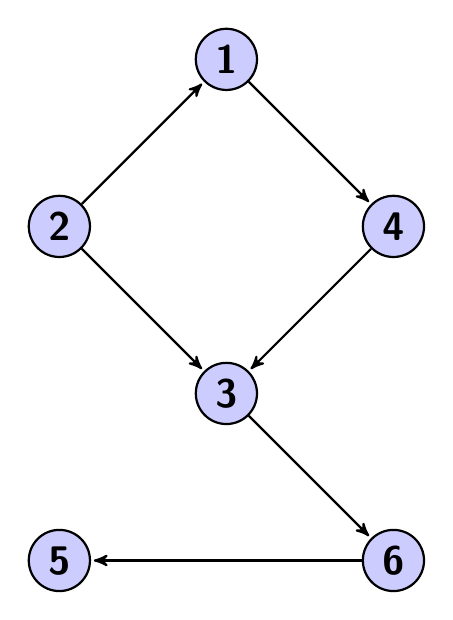
\begin{tikzpicture}[->,>=stealth',shorten >=1pt,auto,node distance=3cm,
  thick,main node/.style={circle,fill=blue!20,draw,font=\sffamily\Large\bfseries}]

  \node[main node] (1) {1};
  \node[main node] (2) [below left of=1] {2};
  \node[main node] (3) [below right of=2] {3};
  \node[main node] (4) [below right of=1] {4};
  \node[main node] (5) [below left of=3] {5};  
  \node[main node] (6) [below right of=3] {6};

  \path[every node/.style={font=\sffamily\small}]
    (1) edge node [left] {} (4)
    (2) edge node [right] {} (1)
        edge [right] node[left] {} (3)
    (3) edge node [right] {} (6)
    (4) edge node [left] {} (3)
    (6) edge node [right] {} (5);
\end{tikzpicture}



\vspace{2cm}
% arbre_dfs.png



\tikzset{
  treenode/.style = {align=center, inner sep=0pt, text centered,
    font=\sffamily},
  arn_n/.style = {treenode, circle, black, font=\sffamily\bfseries, draw=black,
    fill=white, text width=1.5em},
  arn_r/.style = {treenode, circle, black, font=\sffamily\bfseries, draw=black,
    fill=white, text width=1.5em},
  arn_x/.style = {treenode, circle, black, font=\sffamily\bfseries, draw=black,
    fill=white, text width=1.5em},
}
\begin{tikzpicture}[->,>=stealth',level/.style={sibling distance = 5cm/#1,
  level distance = 1.5cm}] 
\node [arn_n] {1}
    child{ node [arn_r] {2} 
            child{ node [arn_n] {3}}
            child{ node [arn_n] {4}
							child{ node [arn_r] {5}}
							child{ node [arn_x] {6}}
            }                            
    }
    child{ node [arn_r] {7}
            child{ node [arn_n] {8} 
							child{ node [arn_r] {9}}
							child{ node [arn_r] {10}}
            }
		}
; 
\end{tikzpicture}

\vspace{2cm}
% graphe_dfs.png

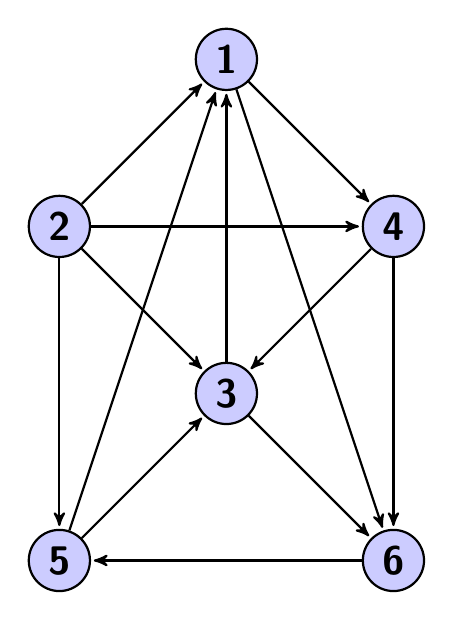
\begin{tikzpicture}[->,>=stealth',shorten >=1pt,auto,node distance=3cm,
  thick,main node/.style={circle,fill=blue!20,draw,font=\sffamily\Large\bfseries}]

  \node[main node] (1) {1};
  \node[main node] (2) [below left of=1] {2};
  \node[main node] (3) [below right of=2] {3};
  \node[main node] (4) [below right of=1] {4};
  \node[main node] (5) [below left of=3] {5};  
  \node[main node] (6) [below right of=3] {6};

  \path[every node/.style={font=\sffamily\small}]
    (1) edge node [left] {} (4)
        edge node [left] {} (6)
    (2) edge node [right] {} (1)
        edge node {} (4)
        edge [right] node[left] {} (3)
        edge node [right] {} (5)
    (3) edge node [right] {} (1)
        edge node [right] {} (6)
    (4) edge node [left] {} (3)
        edge node [right] {} (6)
    (5) edge node [right] {} (1)
        edge node [right] {} (3)
    (6) edge node [right] {} (5);
\end{tikzpicture}


\end{document}